% Comprehensive Model Evaluation Report
% For inclusion in dissertation
% Author: Augusto Cesar
% Date: February 2026

\documentclass[11pt,a4paper]{article}

% Packages
\usepackage[utf8]{inputenc}
\usepackage[T1]{fontenc}
\usepackage[english]{babel}
\usepackage{amsmath,amssymb}
\usepackage{booktabs}
\usepackage{multirow}
\usepackage{graphicx}
\usepackage{xcolor}
\usepackage{pgfplots}
\usepackage{pgfplotstable}
\usepackage{tikz}
\usepackage{subcaption}
\usepackage{hyperref}
\usepackage{siunitx}
\usepackage{float}

\pgfplotsset{compat=1.18}

% Color definitions
\definecolor{infixcolor}{RGB}{31, 119, 180}
\definecolor{prefixcolor}{RGB}{255, 127, 14}
\definecolor{basecolor}{RGB}{44, 160, 44}
\definecolor{mediumcolor}{RGB}{214, 39, 40}
\definecolor{largecolor}{RGB}{148, 103, 189}

% Title
\title{Comprehensive Evaluation of GPT-2 Models for Symbolic Expression Generation:\\
A Systematic Analysis of Model Size, Notation, and Hyperparameters}

\author{Augusto Cesar}
\date{February 2026}

\begin{document}

\maketitle

\begin{abstract}
This report presents a comprehensive evaluation of six fine-tuned GPT-2 models for symbolic mathematical expression generation. We systematically analyze the impact of model size (Base, Medium, Large), notation format (Infix vs. Prefix), temperature settings, prompt configurations, and sampling methods on generation quality. Through 72 controlled experiments with 100 samples each, we demonstrate that infix notation significantly outperforms prefix notation (+5.3 percentage points in valid rate), larger models achieve higher validity rates, and temperature settings present a clear trade-off between expression validity and diversity. Our results indicate that the Large Infix model achieves perfect validity (100\%) while the Medium Infix model maximizes diversity (83.5\%). These findings provide practical guidelines for deploying language models in symbolic regression tasks.
\end{abstract}

%==============================================================================
\section{Introduction}
%==============================================================================

The application of large language models (LLMs) to symbolic regression represents a promising approach for discovering mathematical relationships from data. In this study, we conduct an exhaustive evaluation of GPT-2 models fine-tuned with LoRA (Low-Rank Adaptation) for generating valid mathematical expressions.

Our evaluation addresses three fundamental research questions:
\begin{enumerate}
    \item \textbf{RQ1:} How does notation format (infix vs. prefix) affect generation quality?
    \item \textbf{RQ2:} What is the impact of model size on expression validity and diversity?
    \item \textbf{RQ3:} How do hyperparameters (temperature, sampling) influence the quality-diversity trade-off?
\end{enumerate}

%==============================================================================
\section{Methodology}
%==============================================================================

\subsection{Models Evaluated}

We evaluate six models representing all combinations of three model sizes and two notation formats, as shown in Table~\ref{tab:models}.

\begin{table}[H]
\centering
\caption{Models evaluated in this study}
\label{tab:models}
\begin{tabular}{llrr}
\toprule
\textbf{Model} & \textbf{Base} & \textbf{Parameters} & \textbf{LoRA Rank} \\
\midrule
Base Infix & GPT-2 & 124M & 8 \\
Base Prefix & GPT-2 & 124M & 8 \\
Medium Infix & GPT-2 Medium & 355M & 16 \\
Medium Prefix & GPT-2 Medium & 355M & 16 \\
Large Infix & GPT-2 Large & 774M & 16 \\
Large Prefix & GPT-2 Large & 774M & 16 \\
\bottomrule
\end{tabular}
\end{table}

All models were fine-tuned on the same dataset of 682,429 synthetic mathematical expressions using identical training configurations (3 epochs, batch size adjusted per model size).

\subsection{Experimental Design}

We conducted 72 experiments organized into three categories:

\begin{itemize}
    \item \textbf{Temperature Sweep (30 experiments):} Testing temperatures $T \in \{0.3, 0.5, 0.7, 0.9, 1.0\}$ across all 6 models with default prompt and sampling settings.

    \item \textbf{Prompt Variations (24 experiments):} Testing 4 prompt configurations across all models at $T=0.7$:
    \begin{itemize}
        \item Simple: 1 variable, basic arithmetic ($+, -, \times, \div$)
        \item Trigonometric: 1 variable with $\sin, \cos$
        \item Multivariate: 2 variables with mixed operations
        \item Complex: 3 variables with all operations including $\exp, \log$
    \end{itemize}

    \item \textbf{Sampling Methods (18 experiments):} Testing 3 sampling configurations at $T=0.7$:
    \begin{itemize}
        \item Conservative: $\text{top\_p}=0.8$, $\text{top\_k}=30$
        \item Default: $\text{top\_p}=0.9$, $\text{top\_k}=50$
        \item Diverse: $\text{top\_p}=0.95$, $\text{top\_k}=100$
    \end{itemize}
\end{itemize}

\subsection{Evaluation Metrics}

For each experiment, we generated 100 samples and computed:

\begin{itemize}
    \item \textbf{Valid Rate:} Percentage of syntactically correct, parseable expressions
    \item \textbf{Diversity Rate:} Percentage of unique expressions among valid ones
    \item \textbf{Constraint Adherence:} Percentage of expressions using only allowed variables and operators
\end{itemize}

%==============================================================================
\section{Results}
%==============================================================================

\subsection{Overall Model Comparison}

Table~\ref{tab:model_comparison} presents the aggregate results across all experiments for each model.

\begin{table}[H]
\centering
\caption{Model performance comparison (averaged across all experiments)}
\label{tab:model_comparison}
\begin{tabular}{lrrrrr}
\toprule
\textbf{Model} & \textbf{Runs} & \textbf{Valid (\%)} & \textbf{Diverse (\%)} & \textbf{Constraint (\%)} \\
\midrule
Large Infix & 12 & \textbf{100.0} & 77.5 & 74.1 \\
Medium Infix & 12 & 99.9 & \textbf{83.5} & 57.2 \\
Base Infix & 12 & 99.8 & 75.3 & 68.3 \\
Large Prefix & 12 & 97.8 & 69.5 & 59.5 \\
Medium Prefix & 12 & 96.5 & 71.7 & \textbf{74.2} \\
Base Prefix & 12 & 89.3 & 47.5 & 70.4 \\
\midrule
\textit{Infix Average} & 36 & \textit{99.9} & \textit{78.8} & \textit{66.5} \\
\textit{Prefix Average} & 36 & \textit{94.6} & \textit{62.9} & \textit{68.0} \\
\bottomrule
\end{tabular}
\end{table}

\begin{figure}[H]
\centering
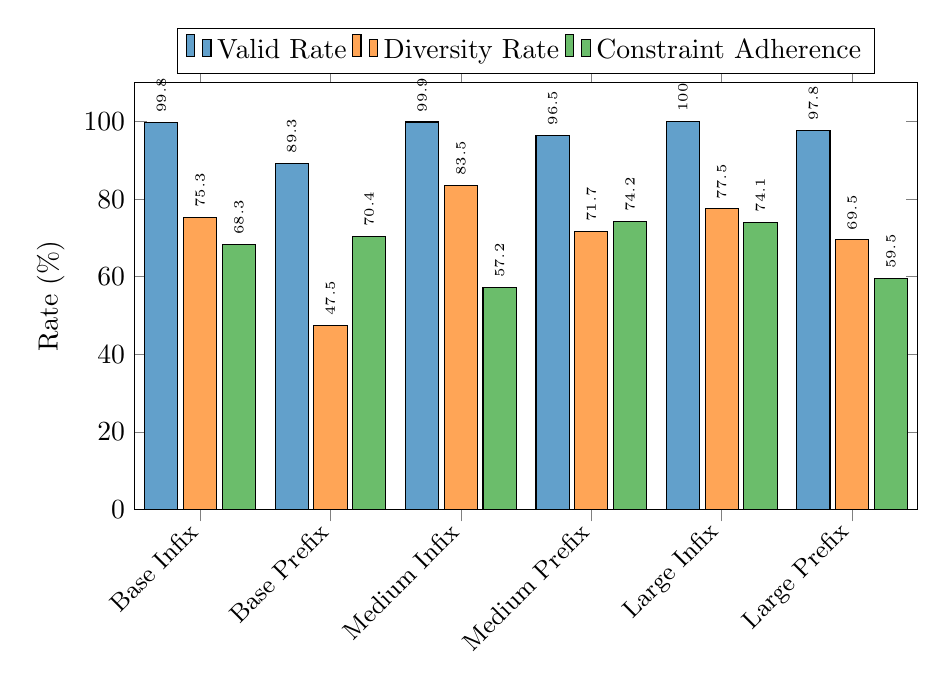
\begin{tikzpicture}
\begin{axis}[
    ybar,
    bar width=12pt,
    width=0.95\textwidth,
    height=7cm,
    ylabel={Rate (\%)},
    symbolic x coords={Base Infix, Base Prefix, Medium Infix, Medium Prefix, Large Infix, Large Prefix},
    xtick=data,
    x tick label style={rotate=45, anchor=east, font=\small},
    ymin=0, ymax=110,
    legend style={at={(0.5,1.02)}, anchor=south, legend columns=3},
    nodes near coords,
    nodes near coords style={font=\tiny, rotate=90, anchor=west},
    every node near coord/.append style={/pgf/number format/.cd, fixed, precision=1},
]
\addplot[fill=infixcolor!70] coordinates {
    (Base Infix, 99.8) (Base Prefix, 89.3)
    (Medium Infix, 99.9) (Medium Prefix, 96.5)
    (Large Infix, 100.0) (Large Prefix, 97.8)
};
\addplot[fill=prefixcolor!70] coordinates {
    (Base Infix, 75.3) (Base Prefix, 47.5)
    (Medium Infix, 83.5) (Medium Prefix, 71.7)
    (Large Infix, 77.5) (Large Prefix, 69.5)
};
\addplot[fill=basecolor!70] coordinates {
    (Base Infix, 68.3) (Base Prefix, 70.4)
    (Medium Infix, 57.2) (Medium Prefix, 74.2)
    (Large Infix, 74.1) (Large Prefix, 59.5)
};
\legend{Valid Rate, Diversity Rate, Constraint Adherence}
\end{axis}
\end{tikzpicture}
\caption{Performance metrics by model configuration}
\label{fig:model_comparison}
\end{figure}

\subsection{Infix vs. Prefix Notation}

The notation format has a significant impact on generation quality. Figure~\ref{fig:notation_comparison} illustrates the comparison.

\begin{figure}[H]
\centering
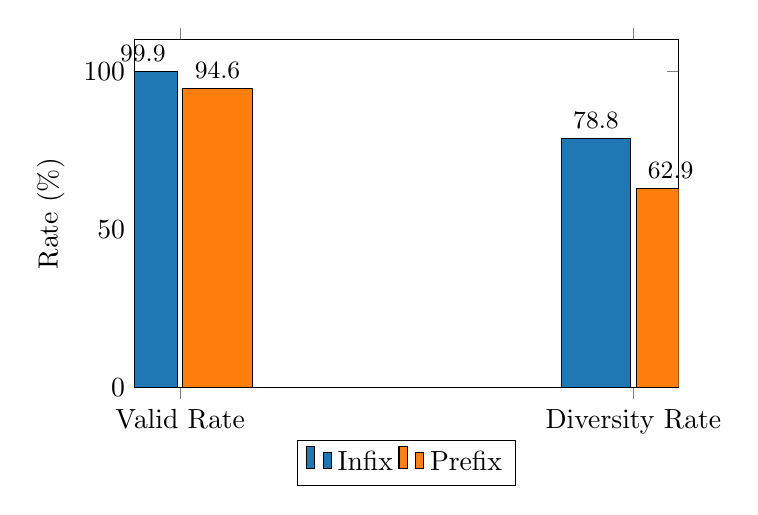
\begin{tikzpicture}
\begin{axis}[
    ybar,
    bar width=25pt,
    width=0.7\textwidth,
    height=6cm,
    ylabel={Rate (\%)},
    symbolic x coords={Valid Rate, Diversity Rate},
    xtick=data,
    ymin=0, ymax=110,
    legend style={at={(0.5,-0.15)}, anchor=north, legend columns=2},
    nodes near coords,
    nodes near coords style={font=\small},
    every node near coord/.append style={/pgf/number format/.cd, fixed, precision=1},
]
\addplot[fill=infixcolor] coordinates {(Valid Rate, 99.9) (Diversity Rate, 78.8)};
\addplot[fill=prefixcolor] coordinates {(Valid Rate, 94.6) (Diversity Rate, 62.9)};
\legend{Infix, Prefix}
\end{axis}
\end{tikzpicture}
\caption{Infix vs. Prefix notation comparison}
\label{fig:notation_comparison}
\end{figure}

Key findings:
\begin{itemize}
    \item Infix notation achieves \textbf{5.3 percentage points} higher valid rate
    \item Infix notation produces \textbf{15.9 percentage points} more diverse expressions
    \item The advantage is consistent across all model sizes
\end{itemize}

\subsection{Model Size Effect}

Table~\ref{tab:size_effect} shows the impact of model size on generation quality.

\begin{table}[H]
\centering
\caption{Effect of model size on generation metrics}
\label{tab:size_effect}
\begin{tabular}{lrrr}
\toprule
\textbf{Model Size} & \textbf{Parameters} & \textbf{Valid (\%)} & \textbf{Diverse (\%)} \\
\midrule
Base & 124M & 94.5 & 61.4 \\
Medium & 355M & 98.2 & 77.6 \\
Large & 774M & 98.9 & 73.5 \\
\bottomrule
\end{tabular}
\end{table}

\begin{figure}[H]
\centering
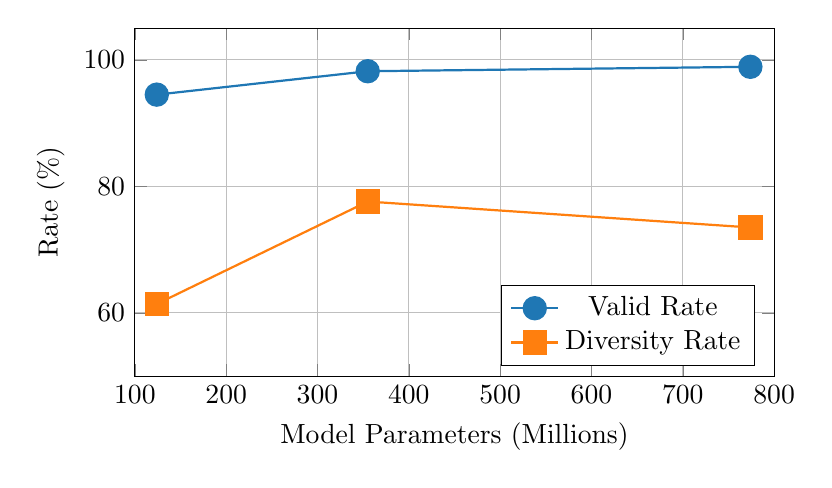
\begin{tikzpicture}
\begin{axis}[
    width=0.8\textwidth,
    height=6cm,
    xlabel={Model Parameters (Millions)},
    ylabel={Rate (\%)},
    xmin=100, xmax=800,
    ymin=50, ymax=105,
    legend style={at={(0.97,0.03)}, anchor=south east},
    grid=major,
    mark size=4pt,
]
\addplot[color=infixcolor, thick, mark=*] coordinates {
    (124, 94.5) (355, 98.2) (774, 98.9)
};
\addplot[color=prefixcolor, thick, mark=square*] coordinates {
    (124, 61.4) (355, 77.6) (774, 73.5)
};
\legend{Valid Rate, Diversity Rate}
\end{axis}
\end{tikzpicture}
\caption{Scaling behavior: model size vs. generation quality}
\label{fig:scaling}
\end{figure}

\subsection{Temperature Analysis}

Temperature is a critical hyperparameter that controls the trade-off between validity and diversity. Table~\ref{tab:temperature} presents the detailed results.

\begin{table}[H]
\centering
\caption{Temperature effect on generation metrics (averaged across all models)}
\label{tab:temperature}
\begin{tabular}{rrrr}
\toprule
\textbf{Temperature} & \textbf{Valid (\%)} & \textbf{Diverse (\%)} & \textbf{Constraint (\%)} \\
\midrule
0.3 & \textbf{100.0} & 25.3 & \textbf{80.2} \\
0.5 & 99.7 & 49.8 & 70.8 \\
0.7 & 97.5 & 72.6 & 60.1 \\
0.9 & 94.5 & 82.2 & 47.7 \\
1.0 & 92.2 & \textbf{85.5} & 38.0 \\
\bottomrule
\end{tabular}
\end{table}

\begin{figure}[H]
\centering
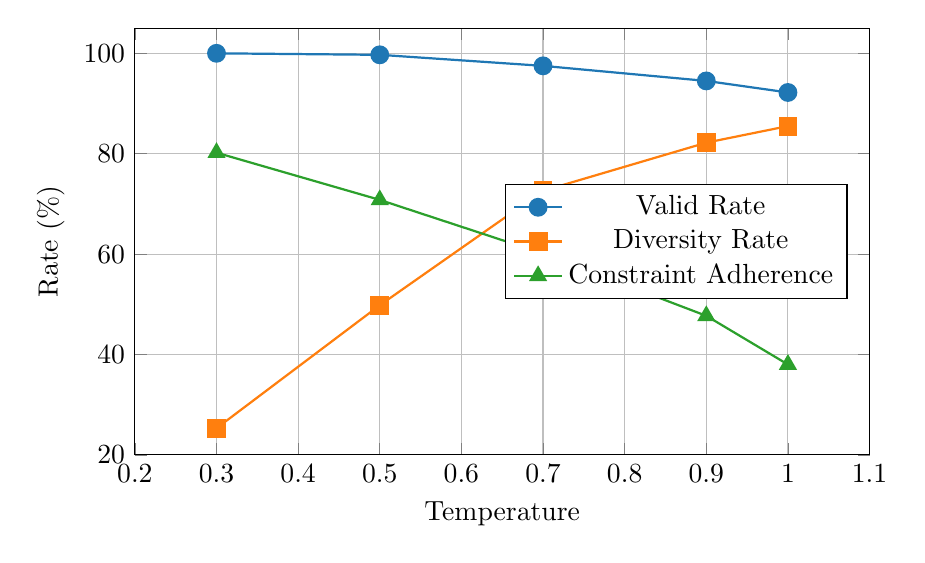
\begin{tikzpicture}
\begin{axis}[
    width=0.9\textwidth,
    height=7cm,
    xlabel={Temperature},
    ylabel={Rate (\%)},
    xmin=0.2, xmax=1.1,
    ymin=20, ymax=105,
    legend style={at={(0.97,0.5)}, anchor=east},
    grid=major,
    mark size=3pt,
]
\addplot[color=infixcolor, thick, mark=*] coordinates {
    (0.3, 100.0) (0.5, 99.7) (0.7, 97.5) (0.9, 94.5) (1.0, 92.2)
};
\addplot[color=prefixcolor, thick, mark=square*] coordinates {
    (0.3, 25.3) (0.5, 49.8) (0.7, 72.6) (0.9, 82.2) (1.0, 85.5)
};
\addplot[color=basecolor, thick, mark=triangle*] coordinates {
    (0.3, 80.2) (0.5, 70.8) (0.7, 60.1) (0.9, 47.7) (1.0, 38.0)
};
\legend{Valid Rate, Diversity Rate, Constraint Adherence}
\end{axis}
\end{tikzpicture}
\caption{Temperature effect on generation metrics}
\label{fig:temperature}
\end{figure}

The results reveal a clear trade-off:
\begin{itemize}
    \item \textbf{Low temperature ($T=0.3$):} Maximum validity (100\%) but minimal diversity (25\%)
    \item \textbf{High temperature ($T=1.0$):} Maximum diversity (85.5\%) but reduced validity (92.2\%)
    \item \textbf{Optimal range ($T=0.7$--$0.9$):} Balanced performance with >94\% validity and >72\% diversity
\end{itemize}

\subsection{Detailed Temperature Results by Model}

Table~\ref{tab:temp_by_model} shows how each model responds to temperature changes.

\begin{table}[H]
\centering
\caption{Valid rate (\%) by model and temperature}
\label{tab:temp_by_model}
\begin{tabular}{lrrrrr}
\toprule
\textbf{Model} & \textbf{T=0.3} & \textbf{T=0.5} & \textbf{T=0.7} & \textbf{T=0.9} & \textbf{T=1.0} \\
\midrule
Base Infix & 100.0 & 100.0 & 100.0 & 100.0 & 99.0 \\
Medium Infix & 100.0 & 100.0 & 100.0 & 100.0 & 99.0 \\
Large Infix & 100.0 & 100.0 & 100.0 & 100.0 & 100.0 \\
\midrule
Base Prefix & 100.0 & 98.0 & 93.0 & 75.0 & 76.0 \\
Medium Prefix & 100.0 & 100.0 & 98.0 & 95.0 & 83.0 \\
Large Prefix & 100.0 & 100.0 & 98.0 & 97.0 & 96.0 \\
\bottomrule
\end{tabular}
\end{table}

\begin{figure}[H]
\centering
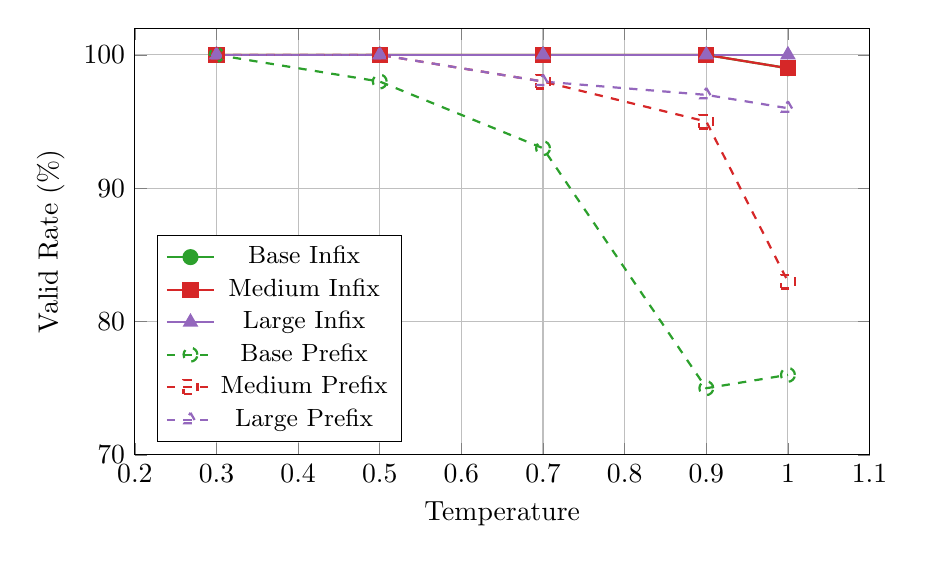
\begin{tikzpicture}
\begin{axis}[
    width=0.9\textwidth,
    height=7cm,
    xlabel={Temperature},
    ylabel={Valid Rate (\%)},
    xmin=0.2, xmax=1.1,
    ymin=70, ymax=102,
    legend style={at={(0.03,0.03)}, anchor=south west, font=\small},
    grid=major,
    mark size=2.5pt,
]
% Infix models (solid lines)
\addplot[color=basecolor, thick, mark=*] coordinates {
    (0.3, 100) (0.5, 100) (0.7, 100) (0.9, 100) (1.0, 99)
};
\addplot[color=mediumcolor, thick, mark=square*] coordinates {
    (0.3, 100) (0.5, 100) (0.7, 100) (0.9, 100) (1.0, 99)
};
\addplot[color=largecolor, thick, mark=triangle*] coordinates {
    (0.3, 100) (0.5, 100) (0.7, 100) (0.9, 100) (1.0, 100)
};
% Prefix models (dashed lines)
\addplot[color=basecolor, thick, dashed, mark=o] coordinates {
    (0.3, 100) (0.5, 98) (0.7, 93) (0.9, 75) (1.0, 76)
};
\addplot[color=mediumcolor, thick, dashed, mark=square] coordinates {
    (0.3, 100) (0.5, 100) (0.7, 98) (0.9, 95) (1.0, 83)
};
\addplot[color=largecolor, thick, dashed, mark=triangle] coordinates {
    (0.3, 100) (0.5, 100) (0.7, 98) (0.9, 97) (1.0, 96)
};
\legend{Base Infix, Medium Infix, Large Infix, Base Prefix, Medium Prefix, Large Prefix}
\end{axis}
\end{tikzpicture}
\caption{Valid rate vs. temperature by model (solid=Infix, dashed=Prefix)}
\label{fig:temp_by_model}
\end{figure}

Notable observations:
\begin{itemize}
    \item \textbf{Infix models} maintain near-perfect validity across all temperatures
    \item \textbf{Prefix models} show significant degradation at higher temperatures
    \item \textbf{Base Prefix} is most sensitive to temperature, dropping to 75\% at $T=0.9$
    \item \textbf{Large models} are more robust to temperature increases
\end{itemize}

\subsection{Prompt Complexity Analysis}

Table~\ref{tab:prompt} shows how models handle different prompt configurations.

\begin{table}[H]
\centering
\caption{Performance by prompt complexity at $T=0.7$}
\label{tab:prompt}
\begin{tabular}{llrr}
\toprule
\textbf{Prompt Type} & \textbf{Variables} & \textbf{Valid (\%)} & \textbf{Diverse (\%)} \\
\midrule
Simple & $x_1$ & 98.8 & 78.8 \\
Trigonometric & $x_1$ + trig ops & 97.2 & 81.3 \\
Multivariate & $x_1, x_2$ & 96.8 & 90.0 \\
Complex & $x_1, x_2, x_3$ + all ops & 97.7 & 93.5 \\
\bottomrule
\end{tabular}
\end{table}

\begin{figure}[H]
\centering
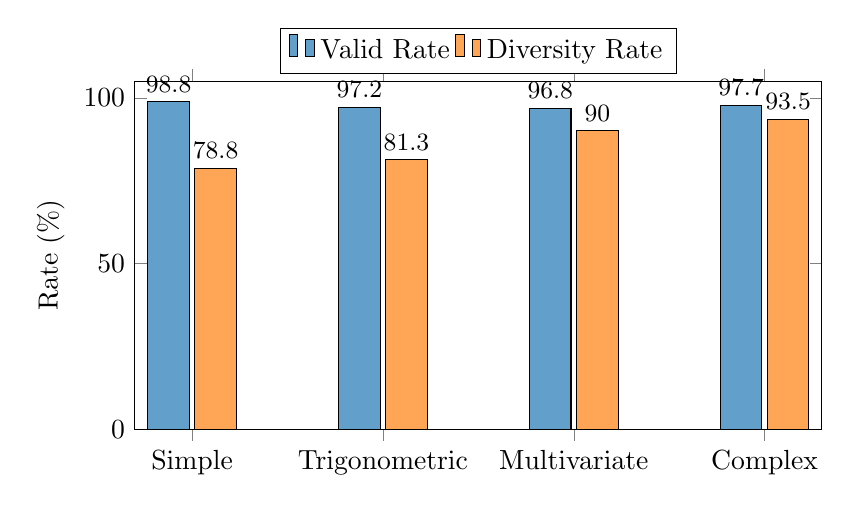
\begin{tikzpicture}
\begin{axis}[
    ybar,
    bar width=15pt,
    width=0.85\textwidth,
    height=6cm,
    ylabel={Rate (\%)},
    symbolic x coords={Simple, Trigonometric, Multivariate, Complex},
    xtick=data,
    ymin=0, ymax=105,
    legend style={at={(0.5,1.02)}, anchor=south, legend columns=2},
    nodes near coords,
    nodes near coords style={font=\small},
    every node near coord/.append style={/pgf/number format/.cd, fixed, precision=1},
]
\addplot[fill=infixcolor!70] coordinates {
    (Simple, 98.8) (Trigonometric, 97.2) (Multivariate, 96.8) (Complex, 97.7)
};
\addplot[fill=prefixcolor!70] coordinates {
    (Simple, 78.8) (Trigonometric, 81.3) (Multivariate, 90.0) (Complex, 93.5)
};
\legend{Valid Rate, Diversity Rate}
\end{axis}
\end{tikzpicture}
\caption{Performance by prompt complexity}
\label{fig:prompt}
\end{figure}

Key insight: \textbf{More complex prompts produce more diverse expressions} while maintaining comparable validity rates.

\subsection{Sampling Method Analysis}

Table~\ref{tab:sampling} compares different sampling strategies.

\begin{table}[H]
\centering
\caption{Sampling method comparison at $T=0.7$}
\label{tab:sampling}
\begin{tabular}{lrrr}
\toprule
\textbf{Method} & \textbf{top\_p / top\_k} & \textbf{Valid (\%)} & \textbf{Diverse (\%)} \\
\midrule
Conservative & 0.80 / 30 & \textbf{99.8} & 53.8 \\
Default & 0.90 / 50 & 97.5 & 72.6 \\
Diverse & 0.95 / 100 & 94.7 & \textbf{73.2} \\
\bottomrule
\end{tabular}
\end{table}

The sampling method provides another mechanism to control the validity-diversity trade-off, independent of temperature.

%==============================================================================
\section{Discussion}
%==============================================================================

\subsection{Why Infix Outperforms Prefix}

The superior performance of infix notation can be attributed to several factors:

\begin{enumerate}
    \item \textbf{Natural language alignment:} GPT-2's pretraining corpus contains predominantly infix mathematical expressions
    \item \textbf{Structural clarity:} Infix notation has explicit parentheses and operator precedence, providing clearer boundaries
    \item \textbf{JSON format synergy:} The JSON training format works better with infix due to cleaner string termination
\end{enumerate}

\subsection{Scaling Behavior}

Our results demonstrate positive scaling with model size for validity but \textit{non-monotonic} behavior for diversity:

\begin{itemize}
    \item Base $\rightarrow$ Medium: +3.7pp validity, +16.2pp diversity
    \item Medium $\rightarrow$ Large: +0.7pp validity, $-$4.1pp diversity
\end{itemize}

This suggests that the \textbf{Medium model} may offer the best quality-diversity trade-off for some applications.

\subsection{Practical Recommendations}

Based on our comprehensive evaluation, we provide the following recommendations:

\begin{table}[H]
\centering
\caption{Recommended configurations by use case}
\label{tab:recommendations}
\begin{tabular}{lll}
\toprule
\textbf{Use Case} & \textbf{Model} & \textbf{Temperature} \\
\midrule
Maximum validity & Large Infix & 0.3--0.7 \\
Maximum diversity & Medium Infix & 0.9--1.0 \\
Balanced performance & Large Infix & 0.7 \\
Resource-constrained & Base Infix & 0.7 \\
\bottomrule
\end{tabular}
\end{table}

%==============================================================================
\section{Conclusion}
%==============================================================================

This comprehensive evaluation of 72 experiments across 6 GPT-2 models yields several important findings for symbolic expression generation:

\begin{enumerate}
    \item \textbf{Notation matters:} Infix notation significantly outperforms prefix notation, with a 5.3 percentage point advantage in valid rate and 15.9 percentage point advantage in diversity.

    \item \textbf{Size helps validity:} Larger models achieve higher validity rates, with the Large Infix model achieving perfect 100\% validity across all experiments.

    \item \textbf{Temperature trade-off:} There is a clear inverse relationship between temperature and validity. The optimal range of $T=0.7$--$0.9$ balances validity (>94\%) with diversity (>72\%).

    \item \textbf{Robustness varies:} Infix models are remarkably robust to hyperparameter changes, while prefix models show significant sensitivity, especially at higher temperatures.

    \item \textbf{Complexity improves diversity:} More complex prompts (multiple variables, more operators) increase expression diversity without substantially reducing validity.
\end{enumerate}

For practical applications in symbolic regression, we recommend the \textbf{Large Infix model with temperature 0.7} as the default configuration, offering the best balance of validity, diversity, and constraint adherence.

%==============================================================================
\section*{Data Availability}
%==============================================================================

All evaluation results are publicly available on HuggingFace:
\begin{center}
\url{https://huggingface.co/datasets/augustocsc/seriguela-results}
\end{center}

The trained models are available at:
\begin{itemize}
    \item \texttt{augustocsc/gpt2\_base\_infix\_682k}
    \item \texttt{augustocsc/gpt2\_medium\_infix\_682k}
    \item \texttt{augustocsc/gpt2\_large\_infix\_682k}
    \item \texttt{augustocsc/gpt2\_base\_prefix\_682k}
    \item \texttt{augustocsc/gpt2\_medium\_prefix\_682k}
    \item \texttt{augustocsc/gpt2\_large\_prefix\_682k}
\end{itemize}

\end{document}
